\section{Bestaande Software}
Onze opdracht is het verbeteren en uitbreiden van de 'NedTrain Planner', dat het resultaat is van meerdere projecten door studenten van de TU Delft. In dit hoofdstuk wordt uiteengezet welke software er al bestaat en wat gebruikt gaat worden gedurende het project. Eerst bespreken we de 'NedTrain Planner' zelf, daarna het framework Qt dat gebruikt is voor het implementeren van de tool en ge\"eindigd zal worden met een beschrijving van Google Test en de solvers.

\subsection{NedTrain Planner}
\label{subsec:planner}
De NedTrain Planner bestaat grofweg uit drie componenten, namelijk de gebruikers-interface, een solver en de communicatie tussen die twee. De gebruikers-interface maakt het mogelijk om een probleeminstantie te maken, deze op te laten lossen door de solver en de oplossing te bekijken.

In vorige bachelorprojecten en mastertheses is deze tool steeds verder uitgebreid. De 'OnTrack Scheduler' is een tool met een eenvoudige GUI en een solver die ontwikkeld is door Ronald Evers. Zijn onderzoek in 2010 voor de masterthesis had als doel om een goede solver te bouwen. \cite{ronaldevers2010}

Daarna is in 2011 door Edwin Bruurs en Cis van der Louw een verbeterde gebruikers interface gemaakt.\cite{bep2011nedtrain} Deze verbeteringen waren gebruiksvriendelijker, maar de kwaliteit van de code was volgens het bachelorproject uit 2012 niet goed.\cite{bep2012nedtrain} Deze groep, bestaande uit Erik Ammerlaan, Jan Elffers, Erwin Walraven en Wilco Wisse, heeft in 2012 opnieuw een verbeterde gebruikers-interface gemaakt voor de 'OnTrack Scheduler'. Deze hebben zij de NedTrain planner genoemd.

In deze nieuwe versie is o.a. de gebruikersinterface uitgebreid, kan het oplosproces stap voor stap weergegeven worden en kunnen probleeminstanties gemakkelijk geladen en opgeslagen worden. De interface van de NedTrain planner is te zien in Figuur \ref{fig:plannergui}.

\begin{figure}[!h]
\label{fig:plannergui}
\centering
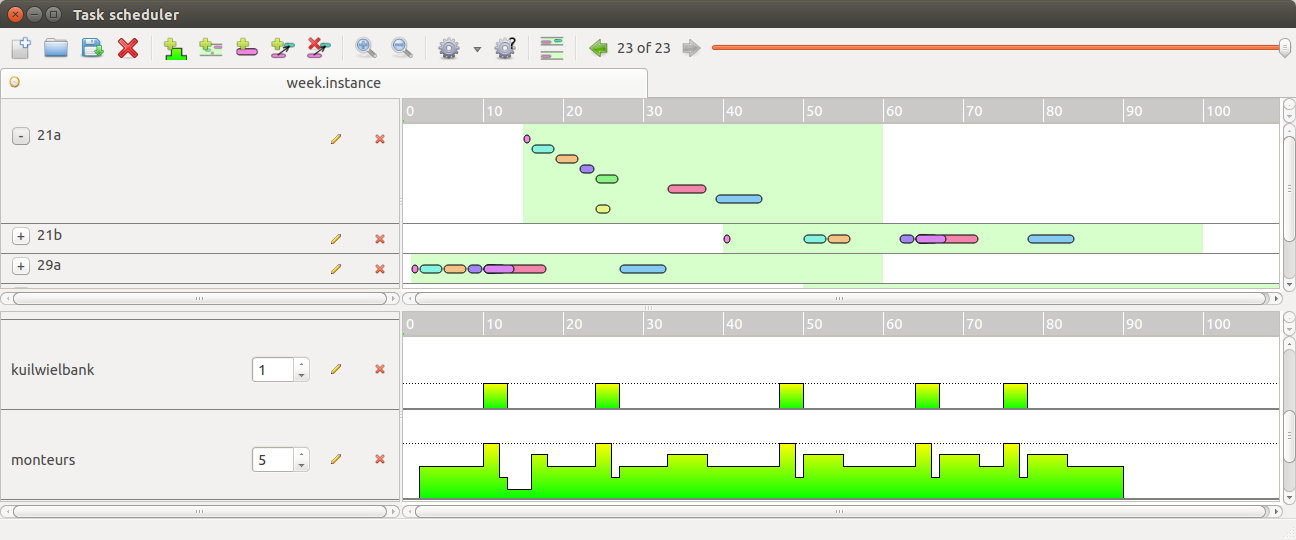
\includegraphics[width=0.8\textwidth]{../images/plannergui.png}
\caption{De gebruikersinterface van de NedTrain planner, zoals deze door het bachelor eindproject in 2012 gemaakt is.}
\end{figure}

\subsection{Qt Framework}
Qt is een gebruikers-interface framework voor \cpp. De NedTrain Planner maakt gebruik van versie 4.8. De nieuwste versie op dit moment is versie 5.2. Door een paar belangrijke veranderingen ge\"introduceerd in versie 5.0, werkt de NedTrain Planner niet meer op versie 5.2. Het updaten van de NedTrain Planner naar deze nieuwe versie zou mogelijk moeten zijn. Qt is open source software die voor meerdere besturingssystemen geschikt is. Het moet dus ook mogelijk zijn om de tool beschikbaar te maken voor o.a. Windows, Linux en Mac OS. Er is een IDE genaamd Qt Creator, die het mogelijk maakt om eenvoudig GUI's te ontwikkelen en \cpp\ code te compileren. \cite{seminarium2014}

\subsection{Google Test}
Voor de bestaande software is er ook testcode geschreven, waarbij gebruik is gemaakt van de Google Test library. Dit maakt het mogelijk om 'unit testing' te doen. Ook ondersteunt de Google Test library fixture, mocks, exceptions, macro's en templates.

\subsection{Solver}
\label{subsec:solver}
%Voor het oplossen van de schedulingsproblemen zijn er twee solvers beschikbaar. De ene is geschreven in python door Michel Wilson en maakt gebruik van een na\"ieve chaining methode die alleen werkt op de Kolisch benchmark-instanties. Op complexere instanties, zoals die van NedTrain, werkt deze solver niet.

Een programma dat een instantie van een schedulingsprobleem oplost wordt een solver genoemd. De solver die wij tot onze beschikking hebben, genaamd TMS, is ontwikkeld door Michel Wilson en is in 2012 verbeterd door de in paragraaf \ref{subsec:planner} genoemde groep voor hun bachelor eindproject. Deze solver maakt gebruik van \emph{Precedence Constraint Posting}, waarbij er voorrangsrelaties aan de taken worden toegevoegd om resource conflicten te verhelpen. \cite{seminarium2014} Deze voorrangsrelaties worden toegevoegd op basis van een heuristiek. Omdat het hier om een NP-compleet probleem gaat, kan het dus zo zijn dat er geen oplossing gevonden wordt, zelfs als deze wel zou bestaan.

Als de solver een oplossing gevonden heeft, worden de taken in de interface zo geplaatst dat er geen enkel resource conflict meer is. De methode die wordt gebruikt, garandeert echter alleen dat de \emph{Earliest Starting Time} oplossing consistent is. Dit betekent dat elke taak op de vroegst mogelijke starttijd begint. In de interface kan er ook met taken geschoven worden, maar dit kan er toe leiden dat er een resource conflict ontstaat. 
